% Rascunho dos slides da defesa do TG (etapa 11). Números retirados de
% thesis/latex/empirical_results.tex, thesis/latex/en/*.tex e dos capítulos de thesis/tg/.
\documentclass[aspectratio=169,11pt]{beamer}
\usepackage[T1]{fontenc}
\usepackage[utf8]{inputenc}
\usepackage{lmodern}
\usepackage{amsmath}
\usepackage{booktabs}
\usepackage{graphicx}

\graphicspath{{../build/figures/}}

% Tema simples: fundo branco, barra de título escura, um acento.
\usetheme{default}
\definecolor{ink}{HTML}{1F2A44}
\definecolor{accent}{HTML}{C8553D}
\definecolor{muted}{HTML}{6B7280}
\setbeamercolor{frametitle}{bg=ink,fg=white}
\setbeamercolor{title}{fg=ink}
\setbeamercolor{subtitle}{fg=muted}
\setbeamercolor{structure}{fg=ink}
\setbeamercolor{alerted text}{fg=accent}
\setbeamercolor{block title}{bg=ink!10,fg=ink}
\setbeamercolor{block body}{bg=ink!4}
\setbeamerfont{frametitle}{series=\bfseries,size=\large}
\setbeamertemplate{navigation symbols}{}
\setbeamertemplate{itemize items}{\color{accent}\textbullet}
\setbeamertemplate{frametitle}{%
  \nointerlineskip
  \begin{beamercolorbox}[wd=\paperwidth,ht=2.6ex,dp=1.2ex,leftskip=1em]{frametitle}
    \usebeamerfont{frametitle}\insertframetitle
  \end{beamercolorbox}}
\setbeamertemplate{footline}{%
  \hfill\usebeamercolor[fg]{subtitle}\scriptsize\insertframenumber\,/\,\inserttotalframenumber
  \hspace*{1em}\vspace*{0.8ex}}

\newcommand{\aself}{\alpha_{\mathrm{self}}}
\newcommand{\across}{\alpha_{\mathrm{cross}}}
\newcommand{\take}[1]{\par\medskip{\color{accent}\bfseries #1}}

\title{Hawkes Process Estimation on High-Frequency\\Cryptocurrency Data via Neural Networks}
\subtitle{Trabalho de Graduação --- Engenharia de Computação, ITA}
\author{João Matheus Del Vecchio França Barbosa\\[0.3ex]
  {\small Advisor: Prof. Dr. Mauri Aparecido de Oliveira (ITA)}}
\date{XX de XXXXX de 2026} % TODO (etapa 12): data da defesa

\begin{document}

\begin{frame}[plain]
  \titlepage
\end{frame}

% ---------------------------------------------------------------- motivation
\begin{frame}{Motivation}
  \begin{itemize}
    \item Price changes cluster: a move tends to be followed by more moves.
    \item The Hawkes process models this self-excitation with few, interpretable parameters.
    \item Estimating it by maximum likelihood (MLE) needs an optimization per window.
    \item \textbf{Amortized estimation}: train a network once on simulated paths; each new
          window then costs a single forward pass (Lee, 2023).
    \item Lee (2023): an LSTM on U.S.\ equities (NBBO data, not public).
  \end{itemize}
  \par\medskip This work: reproduce Lee on public crypto data, test attention, and take the
  estimators to real windows.
\end{frame}

% ---------------------------------------------------------------- model
\begin{frame}{Symmetric bivariate Hawkes process}
  Up-moves \(N_1\) and down-moves \(N_2\), exponential kernel:
  \[
    \lambda_1(t)=\mu+\sum_{t_k^1<t}\aself e^{-\beta(t-t_k^1)}
     +\sum_{t_k^2<t}\across e^{-\beta(t-t_k^2)}
  \]
  and symmetrically for \(\lambda_2\).
  \begin{columns}[T]
    \begin{column}{0.5\textwidth}
      \begin{itemize}
        \item \(\mu\): exogenous activity
        \item \(\aself\): persistence of direction
        \item \(\across\): reversion
        \item \(\beta\): speed of forgetting
      \end{itemize}
    \end{column}
    \begin{column}{0.5\textwidth}
      Stability (branching ratio):
      \[
        g=\frac{\aself+\across}{\beta}<1
      \]
      \(g\to1\): long cascades, near-critical.
    \end{column}
  \end{columns}
\end{frame}

% ---------------------------------------------------------------- question
\begin{frame}{Research question and hypotheses}
  \begin{block}{Question}
    Can an attention-based architecture estimate the parameters of a 2D Hawkes process on
    crypto price moves with accuracy and stability equal to or better than Lee's LSTM,
    while keeping inference faster than the MLE?
  \end{block}
  \medskip
  Registered before the final run:
  \begin{itemize}
    \item \textbf{H1.} Binance's public USD-M data yield sequences structurally equivalent
          to Lee's.
    \item \textbf{H2.} The LSTM reaches MLE-level error with substantially lower latency.
    \item \textbf{H3.} Attention improves error or robustness on long-range dependencies.
  \end{itemize}
\end{frame}

% ---------------------------------------------------------------- data
\begin{frame}{Data: Binance USD-M perpetual futures}
  \begin{columns}[T]
    \begin{column}{0.44\textwidth}
      \begin{itemize}
        \item BTCUSDT and ETHUSDT, \texttt{bookTicker} (best bid/ask)
        \item SHA-256 manifest, audited schema
        \item Mid-price on a \alert{100~ms grid} (last state per bin)
        \item Event = mid-price change (up / down)
        \item Chronological splits, no window crosses a split
      \end{itemize}
    \end{column}
    \begin{column}{0.54\textwidth}
      \footnotesize
      \begin{tabular}{lrr}
        \toprule
        Window & Events & Windows\\
        \midrule
        Primary (Jan.\ 2024) & 1,826,904 & 1,813\\
        Robustness (Oct.\ 2023) & 1,288,352 & 1,281\\
        \bottomrule
      \end{tabular}
      \par\medskip
      Calibration block (15--22 Jan.):
      \begin{itemize}
        \item 76\% of moves repeat direction
        \item median jump 10--15 ticks
        \item 37--39\% of gaps equal the grid step
      \end{itemize}
    \end{column}
  \end{columns}
\end{frame}

% ---------------------------------------------------------------- methods
\begin{frame}{Estimators}
  \begin{columns}[T]
    \begin{column}{0.44\textwidth}
      \textbf{Simulation}: Ogata thinning, empty initial history.
      \par\medskip
      \textbf{Constrained MLE}
      \[
        \begin{aligned}
        (\mu,\aself,\across,d)&=\operatorname{softplus}(z)\\
        \beta&=\aself+\across+d
        \end{aligned}
      \]
      L-BFGS-B, analytic gradient, 5 heuristic starts; never initialized at the truth.
    \end{column}
    \begin{column}{0.54\textwidth}
      \textbf{Networks} (input per event: \((\log(1+\Delta t),\pm1)\); same output head,
      \(g<1\) by construction)
      \par\smallskip
      \footnotesize
      \begin{tabular}{lrr}
        \toprule
         & LSTM & Transformer\\
        \midrule
        Layers & 2 LSTM\(\times\)12 & 2 enc., \(d{=}32\)\\
        Heads / FF & -- & 4 / 128\\
        Parameters & 2,068 & 25,700\\
        Effective batch & 64 & 8\\
        Best epochs & 164--299 & 38--73\\
        Training (5 seeds) & 41 h & 110 h\\
        \bottomrule
      \end{tabular}
    \end{column}
  \end{columns}
\end{frame}

% ---------------------------------------------------------------- protocol
\begin{frame}{Frozen synthetic protocol}
  \begin{itemize}
    \item 75,000 / 10,000 / 15,000 paths, all of 1,000 events
    \item Prior: \(\mu\in[0.2,0.6]\), \(\beta\in[0.8,2.0]\), self-excited fraction
          \(\in[0.2,0.8]\)
    \item \(g\) balanced across three strata: low \([0.10,0.35)\), intermediate
          \([0.35,0.70)\), near-critical \([0.70,0.95]\)
    \item Loss: MSE on the original scale; Adam \(10^{-3}\); 300 epochs, patience 30
    \item 5 seeds per network; MLE fitted on every test path
    \item Test set opened once; tables and figures generated from the artifacts
  \end{itemize}
\end{frame}

% ---------------------------------------------------------------- synthetic results
\begin{frame}{Synthetic results}
  \begin{columns}[T]
    \begin{column}{0.46\textwidth}
      \small
      \begin{tabular}{lrr}
        \toprule
        Estimator & Macro MSE & MSE of \(g\)\\
        \midrule
        LSTM & 0.0196 & 0.0018\\
        Transformer & 0.0237 & 0.0021\\
        MLE & 0.506 & 0.0023\\
        \bottomrule
      \end{tabular}
      \par\medskip
      \begin{itemize}
        \item LSTM vs Transformer: not significant across seeds (Welch \(p=0.19\))
        \item LSTM ensemble better on 70\% of paths, in every \(g\) regime
      \end{itemize}
    \end{column}
    \begin{column}{0.52\textwidth}
      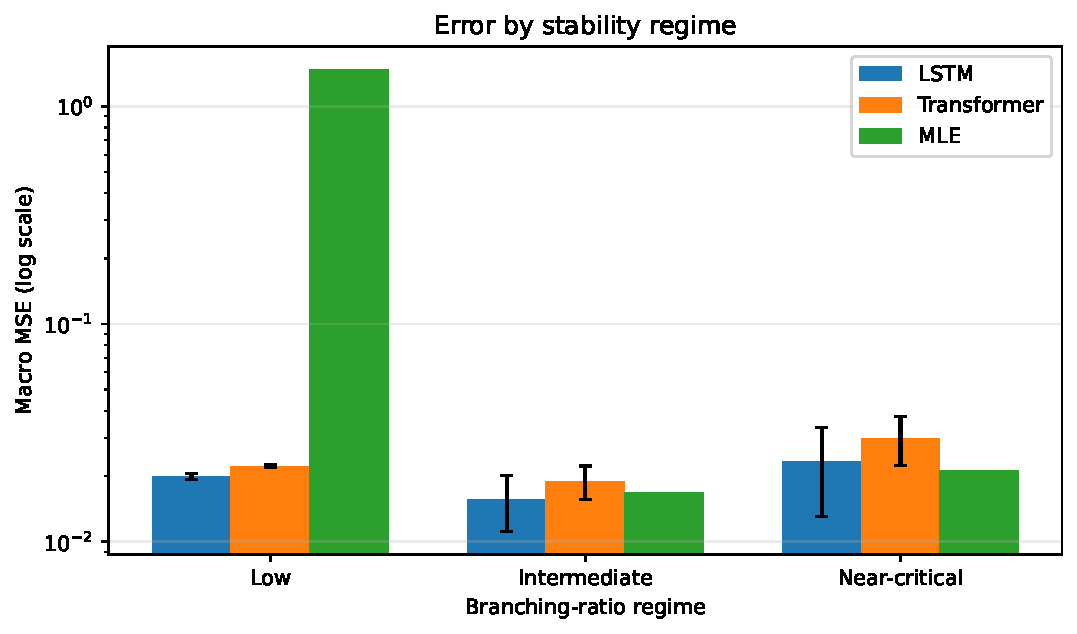
\includegraphics[width=\linewidth]{branching_regime_mse_en.pdf}
    \end{column}
  \end{columns}
\end{frame}

\begin{frame}{Why the MLE ``loses'': identifiability of \(\beta\)}
  \small
  \begin{columns}[T]
    \begin{column}{0.5\textwidth}
      \begin{itemize}
        \item 94\% of the MLE's squared error in \(\beta\) comes from 1\% of the paths,
              almost all with low \(g\)
        \item In all 300 worst paths the likelihood at the estimate \alert{exceeds} the
              likelihood at the truth
      \end{itemize}
    \end{column}
    \begin{column}{0.48\textwidth}
      \begin{itemize}
        \item Networks shrink toward the prior and never leave \(\beta\in[0.8,2.0]\)
        \item Typical path: median loss MLE 0.149 vs LSTM 0.151
      \end{itemize}
    \end{column}
  \end{columns}
  \par\smallskip\centering
  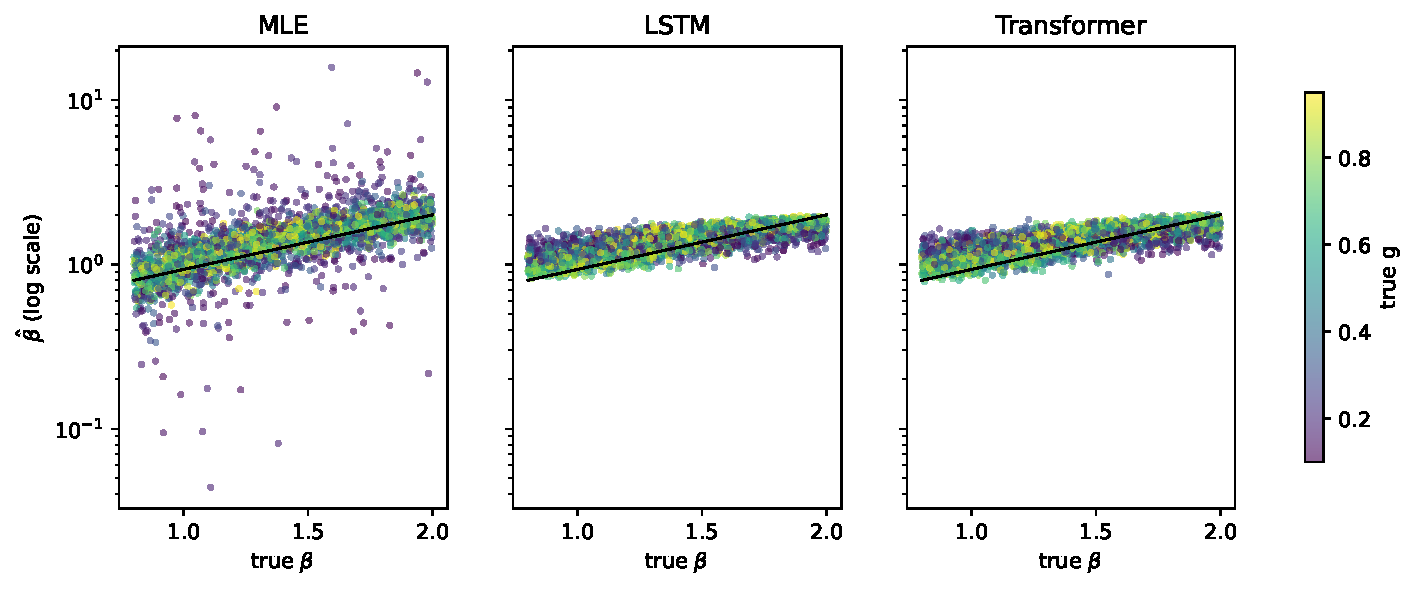
\includegraphics[height=0.52\textheight]{posthoc_beta_verdadeiro_vs_estimado_en.pdf}
\end{frame}

\begin{frame}{Lee's fixed point and computational cost}
  \begin{columns}[T]
    \begin{column}{0.5\textwidth}
      \textbf{Fixed point} \((0.3, 0.4, 0.7, 1.5)\), 2,000 paths
      \begin{itemize}
        \item MLE nearly unbiased; SD \(\approx\sqrt2\times\) Lee's (half the length)
        \item Networks shrink \(\aself,\across\) toward the prior, as in the paper
        \item Macro MSE: MLE 0.0103, LSTM 0.0111
        \item Heuristic and oracle MLE give identical estimates
      \end{itemize}
    \end{column}
    \begin{column}{0.48\textwidth}
      \textbf{Cost per path} (controlled benchmark)
      \par\smallskip
      \footnotesize
      \begin{tabular}{lr}
        \toprule
        MLE, 5 starts, one core & 9.6 ms\\
        LSTM, batch 1, CPU & 7.0 ms\\
        Transformer, batch 1, CPU & 4.8--9.9 ms\\
        LSTM, batch 256, MPS & 0.07 ms\\
        \midrule
        Lee: network / MLE & 12 / 1,763 ms\\
        \bottomrule
      \end{tabular}
      \par\medskip
      Lee's \(\sim\)150\(\times\) gain is not reproduced at batch size one.
    \end{column}
  \end{columns}
\end{frame}

% ---------------------------------------------------------------- real data
\begin{frame}{Real windows lie outside the training prior}
  \small
  MLE on 1,063 calibration windows: median \(\beta=2.71\) (prior: \(\le2.0\));
  \(\across<10^{-3}\) in 89\% of windows; \alert{0\%} of windows inside all prior ranges.
  \par\smallskip\centering
  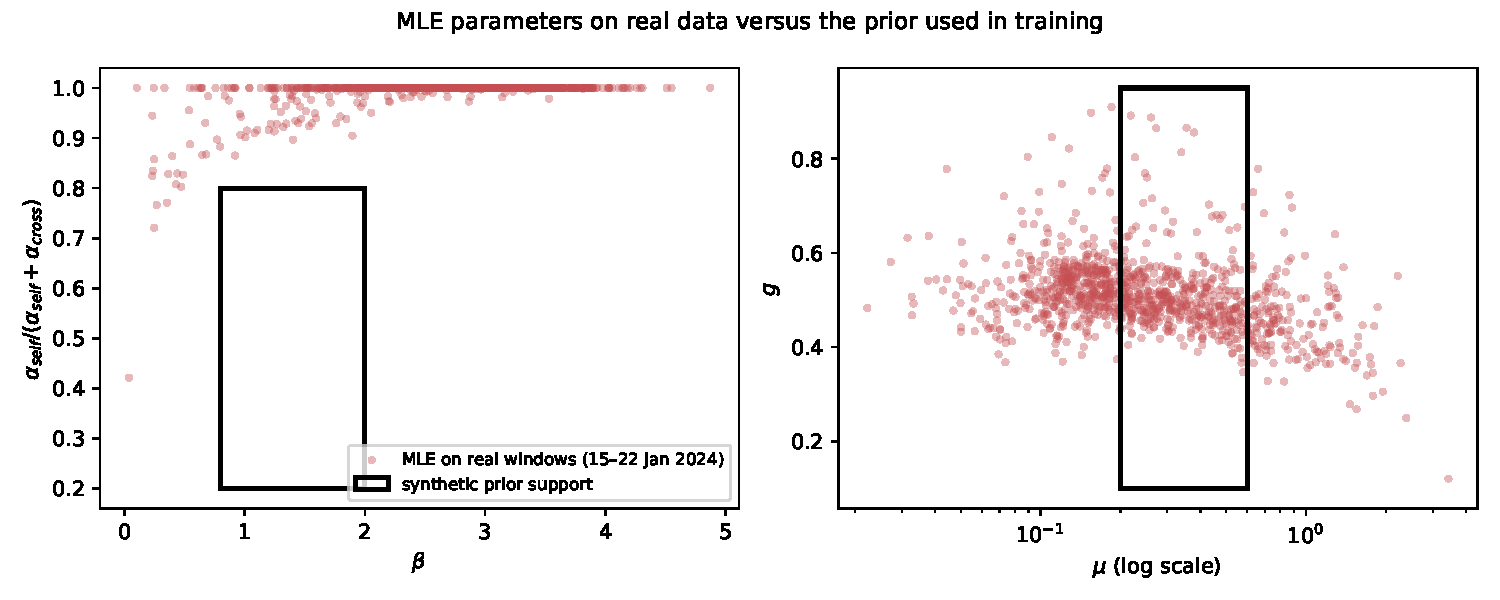
\includegraphics[height=0.55\textheight]{posthoc_calibracao_vs_prior_en.pdf}
  \take{Networks trained on the synthetic prior cannot reach this region.}
\end{frame}

\begin{frame}{Goodness of fit on real data}
  \begin{columns}[T]
    \begin{column}{0.44\textwidth}
      \footnotesize
      \begin{tabular}{lrr}
        \toprule
        Data & KS rej. & LB rej.\\
        \midrule
        Hawkes, real, jittered & 70.3\% & 47.1\%\\
        Simulated on grid & 47.7\% & 4.7\%\\
        Simulated, continuous & 0.9\% & 4.9\%\\
        \bottomrule
      \end{tabular}
    \end{column}
    \begin{column}{0.54\textwidth}
      \footnotesize
      \begin{itemize}
        \item Hawkes \(\gg\) Poisson: LR rejects Poisson in 99.8\%; median \(\Delta\)AIC \(-721\)
        \item The grid alone inflates KS
        \item Ljung--Box keeps its size on the grid, but rejects 47\% on real data
        \item Same pattern on the test block (274 windows): LR 100\%, Ljung--Box 47\% vs 4\%
      \end{itemize}
    \end{column}
  \end{columns}
  \par\smallskip\centering
  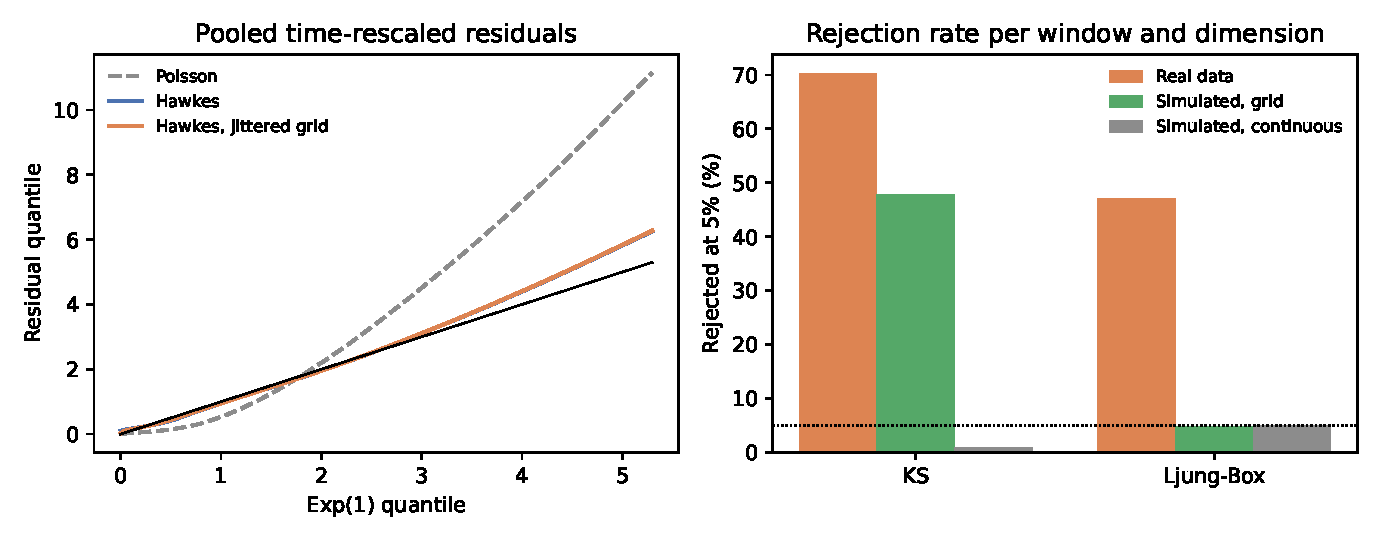
\includegraphics[height=0.39\textheight]{real_data_residual_diagnostics.pdf}
  \take{Target on real data = MLE of an approximating model.}
\end{frame}

\begin{frame}{Networks on real windows (scope A)}
  \small
  Label = MLE of each window. Train 15--22 Jan.\ (1,063), select 23--25 Jan.\ (476),
  test 26--28 Jan.\ (274), opened once. 3.0 h of machine time.
  \par\medskip
  \begin{tabular}{lrrrr}
    \toprule
    Variant (5-seed ensemble) & Validation & \(R^2_\beta\) (val.) & Test & October\\
    \midrule
    Training-label mean & 0.210 & 0.00 & 0.218 & 0.629\\
    LSTM, synthetic weights & 0.555 & \(-1.19\) & 0.250 & 1.115\\
    Transformer, synthetic weights & 0.558 & \(-1.08\) & 0.275 & 1.060\\
    LSTM, from scratch & 0.139 & 0.30 & 0.250 & 0.409\\
    Transformer, from scratch & 0.100 & 0.47 & 0.169 & 0.333\\
    \alert{LSTM, fine-tuned} (selected) & 0.036 & 0.82 & 0.044 & 0.121\\
    Transformer, fine-tuned & 0.041 & 0.79 & 0.040 & 0.083\\
    \bottomrule
  \end{tabular}
  \par\medskip
  Macro MSE against the MLE label. October 2023: never used for training or selection.
\end{frame}

\begin{frame}{Fine-tuned LSTM vs Transformer (post hoc)}
  Paired by window; loss = squared error averaged over the 4 parameters;
  difference = LSTM \(-\) Transformer.
  \par\medskip
  \begin{tabular}{lrrr}
    \toprule
    Block & Difference & Bootstrap 95\% CI & Wilcoxon \(p\)\\
    \midrule
    Test (274 windows) & 0.0046 & \([-0.0020,\ 0.0112]\) & 0.385\\
    October 2023 (1,281) & 0.0384 & \([0.0319,\ 0.0449]\) & \(<10^{-32}\)\\
    \bottomrule
  \end{tabular}
  \par\medskip
  \begin{itemize}
    \item Test: the two variants cannot be told apart
    \item October: the Transformer has the lower loss in 64\% of windows
    \item Not pre-registered: the selection had already been made on validation
  \end{itemize}
  \par\medskip Only the fine-tuned networks are usable; the Transformer degrades less under
  a change of regime.
\end{frame}

\begin{frame}{Hawkes volatility}
  \begin{columns}[T]
    \begin{column}{0.5\textwidth}
      \small
      \[
        \sigma_H^2 = 2\Lambda\Big[\operatorname{Var}(J)+\tfrac{\mathbb E[J]^2}{(1-a_s+a_c)^2}\Big],
        \quad \Lambda=\tfrac{\mu}{1-a_s-a_c}
      \]
      \(J\) = absolute log return per event; compared with the realized volatility of the
      log mid-price sampled every \(\Delta=10\)~s.
      \par\medskip
      Level about right (ratio \(\approx1.25\)); the network ranks windows worse.
      Addendum (Feb 2024): Transformer 0.69, LSTM 0.47, MLE 0.77.
    \end{column}
    \begin{column}{0.46\textwidth}
      \footnotesize
      \begin{tabular}{llrr}
        \toprule
        Block & Params & Ratio & \(\rho_S\)\\
        \midrule
        Validation & MLE & 1.24 & 0.67\\
        Validation & network & 1.24 & 0.47\\
        Test & MLE & 1.27 & 0.78\\
        Test & network & 1.38 & 0.28\\
        \bottomrule
      \end{tabular}
    \end{column}
  \end{columns}
  \par\smallskip\centering
  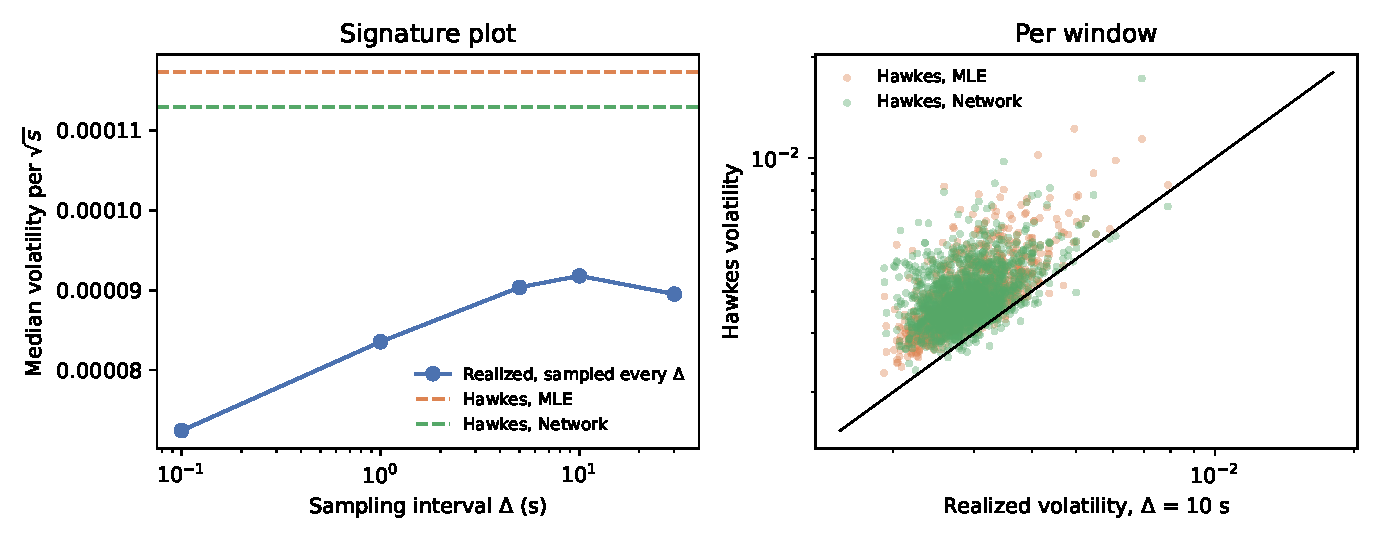
\includegraphics[height=0.38\textheight]{hawkes_volatility.pdf}
\end{frame}

% ---------------------------------------------------------------- addendum
\begin{frame}{Addendum (ADR 009): a new week, read once}
  Same data and seeds; one candidate chosen on validation, then compared with the frozen
  LSTM on 5--11 Feb 2024 (711 windows, never used before).
  \par\medskip
  \footnotesize
  \begin{tabular}{lrrr}
    \toprule
    Candidate & Validation & New week & October\\
    \midrule
    LSTM, frozen (selected in the TG) & 0.0359 & 0.0264 & 0.121\\
    Transformer, frozen & 0.0413 & 0.0285 & 0.083\\
    LSTM, 1,000-epoch cap (\alert{selected}) & \textbf{0.0294} & 0.0212 & 0.116\\
    LSTM, warm-up + plateau decay & 0.0358 & 0.0260 & 0.131\\
    LSTM, standardized loss & 0.0354 & 0.0315 & 0.102\\
    Average LSTM + Transformer & 0.0304 & \textbf{0.0204} & 0.087\\
    \bottomrule
  \end{tabular}
  \par\medskip\small
  \begin{itemize}
    \item Primary: \(-0.0052\), CI \([-0.0060,\,-0.0044]\), lower loss in 73\% of windows
    \item The average also wins (Holm \(p<10^{-12}\)); schedule ties; standardized loss loses
  \end{itemize}
  \par\medskip The LSTM was undertrained; the average of the two networks has the lowest loss on the new week.
\end{frame}

\begin{frame}{Addendum: how much of \(\beta\) the 100~ms grid hides}
  \begin{columns}[T]
    \begin{column}{0.5\textwidth}
      \small
      Simulate in continuous time, take to the grid (one event per cell), fit the MLE;
      invert the median map for each real window.
      \par\medskip
      \begin{itemize}
        \item Grid label \(\approx\) \alert{58\%} of the continuous \(\beta\)
        \item January: 2.71 on the grid \(\leftrightarrow\) 4.7 continuous
        \item October: 3.19 \(\leftrightarrow\) 6.5
        \item Mean memory \(\approx\) 210~ms, not 370~ms
        \item Jitter breaks ties, cannot restore merged events
      \end{itemize}
    \end{column}
    \begin{column}{0.46\textwidth}
      \footnotesize
      \begin{tabular}{lrrr}
        \toprule
        True \(\beta\) & \(\mu=0.05\) & \(0.23\) & \(1.0\)\\
        \midrule
        1.2 & 1.04 & 0.93 & 0.63\\
        2.7 & 2.11 & 1.88 & 1.26\\
        4.5 & 3.17 & 2.72 & 1.83\\
        8.0 & 4.63 & 4.01 & 2.65\\
        13.0 & 5.97 & 5.02 & 3.25\\
        \bottomrule
      \end{tabular}
      \par\smallskip
      Median MLE \(\beta\) on the grid
    \end{column}
  \end{columns}
  \take{The labels describe the process seen through the grid, not in continuous time.}
\end{frame}

\begin{frame}{Addendum (ADR 010): a prior built from the real labels}
  Reduced scope B: invert January labels to continuous time (+ noise, 25\% wide box),
  simulate, take to the grid, label by the MLE; pretrain the LSTM, fine-tune
  (1,000-epoch recipe). Second new week, read once: 4--10 Mar 2024 (1,860 windows).
  \par\medskip
  \footnotesize
  \begin{tabular}{lrrrr}
    \toprule
    Candidate & Validation & March & February & October\\
    \midrule
    LSTM, 1,000-epoch cap (ADR 009) & 0.0294 & 0.109 & 0.0212 & 0.116\\
    Average LSTM + Transformer (ADR 009) & 0.0304 & 0.102 & 0.0204 & 0.087\\
    Scope B LSTM, no fine-tuning & 0.1439 & 0.122 & 0.2115 & 0.141\\
    Scope B LSTM, fine-tuned & 0.0202 & \textbf{0.040} & 0.0153 & \textbf{0.034}\\
    Scope B LSTM + Transformer & \textbf{0.0196} & 0.056 & \textbf{0.0137} & 0.041\\
    \bottomrule
  \end{tabular}
  \par\medskip\small
  \begin{itemize}
    \item Primary: \(-0.068\), CI \([-0.082,\,-0.056]\): \alert{63\% lower loss}, wins in 72\% of windows
    \item Gain is in \(\mu\) (March MSE 0.31 \(\to\) 0.086): extrapolates to higher activity
  \end{itemize}
  \par\medskip A prior built from the real labels helps more than a longer budget; it still needs fine-tuning.
\end{frame}

\begin{frame}{Addendum (ADR 011): can a network undo the grid?}
  LSTM trained on gridded scope B paths with the \alert{continuous-time truth} as target;
  2,000 new paths of the same prior.
  \par\medskip
  \footnotesize
  \begin{tabular}{lrrr}
    \toprule
    Estimator & Macro MSE & Bias \(\beta\) & \(|\)Error\(|\) \(\beta\)\\
    \midrule
    LSTM, trained on the truth & \textbf{0.33} & \(+2.8\%\) & 8.9\%\\
    MLE on the grid & 3.95 & \(-44.1\%\) & 44.1\%\\
    MLE corrected by the map & 0.65 & \(-2.4\%\) & \textbf{8.4\%}\\
    \bottomrule
  \end{tabular}
  \par\medskip\small
  \begin{itemize}
    \item Primary (network vs corrected MLE): \(-0.33\), CI \([-0.40,\,-0.26]\); map better on the typical path
    \item Real windows: network \(\beta\approx7.7\), map 4.9, grid 2.76 (Spearman 0.55): they disagree
  \end{itemize}
  \par\medskip The correction works in simulation but cannot yet be trusted on real windows.
\end{frame}

% ---------------------------------------------------------------- assessment
\begin{frame}{Assessment of the hypotheses}
  \begin{itemize}
    \item H1: \alert{supported} as to structure and volume; but persistent
          direction, multi-tick jumps and grid-discretized times.
    \item H2: \alert{partially supported}. LSTM error of the MLE's order; lower
          latency only in batched inference, not against an efficient MLE at batch size one.
    \item H3: \alert{not supported} on synthetic data: attention did not reduce
          error, not even in the near-critical regime.
    \item Real windows: the fine-tuned networks tie on the test block; the
          fine-tuned Transformer degrades less in October (post hoc); on a pre-registered new
          week the LSTM + Transformer average is best: attention complements the LSTM;
          with a prior built from the real labels, the LSTM alone is best.
  \end{itemize}
\end{frame}

\begin{frame}{Limitations}
  \begin{itemize}
    \item No hyperparameter search; post-LN Transformer without warm-up; batch 8 vs 64
    \item Five seeds; the fine-tuned LSTM stopped near the 300-epoch cap (addendum: a longer
          budget helps)
    \item On real data the label is the MLE of a misspecified model;
          \(\across\) on the boundary of the parameter space; labels biased by the grid
    \item Synthetic metrics depend on a prior not calibrated on the data (scope B: LSTM only,
          one prior design)
    \item Two assets, two windows; latency depends on hardware and batch
    \item Lee's paper omits ranges, seeds and training details
  \end{itemize}
\end{frame}

\begin{frame}{Future work}
  \begin{itemize}
    \item Extend the prior built from the real labels to the Transformer and more weeks
    \item Make the grid correction trustworthy on real data (grid-aware likelihood,
          prior covering the misspecification)
    \item Richer kernels to absorb the residual dependence (sums of exponentials,
          power law)
    \item Transformer: pre-LN, continuous-time encodings, hyperparameter search
          (warm-up and standardized targets did not help in the addendum)
    \item Use the estimators for volatility forecasting, not only description
  \end{itemize}
\end{frame}

\begin{frame}{Conclusion}
  \begin{itemize}
    \item Reproducible pipeline from public Binance data to a frozen comparison of three
          estimators; Lee's qualitative pattern reproduced at the fixed point
    \item Attention brought no accuracy gain on synthetic data
    \item The networks' aggregate-MSE advantage comes from robustness where \(\beta\) is
          poorly identified, and from shrinkage toward the prior
    \item Crypto occupies another region of the parameter space; the networks become usable
          on real windows only with synthetic pretraining plus fine-tuning on MLE labels
    \item Hawkes volatility gets the level right; the MLE ranks windows best
    \item Addendum: longer training and an LSTM + Transformer average beat the selected
          LSTM on a new week; a prior built from the real labels cuts the loss by 63\% on
          another
  \end{itemize}
  \take{Main benefit of amortized estimation: robustness and batched cost, not per-path
  accuracy.}
\end{frame}

\begin{frame}[plain]
  \centering\vfill
  {\Large\bfseries\color{ink} Thank you}
  \par\bigskip
  {\small\color{muted} Code, artifacts and protocol: private repository, release
  \texttt{resultados-finais}}
  \vfill
\end{frame}

% ---------------------------------------------------------------- backup
\appendix
\begin{frame}{Backup: test MSE by parameter (synthetic)}
  \begin{columns}[T]
    \begin{column}{0.44\textwidth}
      \footnotesize
      \setlength{\tabcolsep}{4pt}
      \begin{tabular}{lrrrr}
        \toprule
         & \(\mu\) & \(\aself\) & \(\across\) & \(\beta\)\\
        \midrule
        LSTM & 0.0023 & 0.016 & 0.017 & 0.043\\
        Transf. & 0.0024 & 0.021 & 0.021 & 0.050\\
        MLE & 0.0101 & 0.006 & 0.006 & 2.002\\
        \bottomrule
      \end{tabular}
      \par\medskip
      MLE is best for \(\aself\) and \(\across\); \(\beta\) carries 98.9\% of its
      squared error.
    \end{column}
    \begin{column}{0.54\textwidth}
      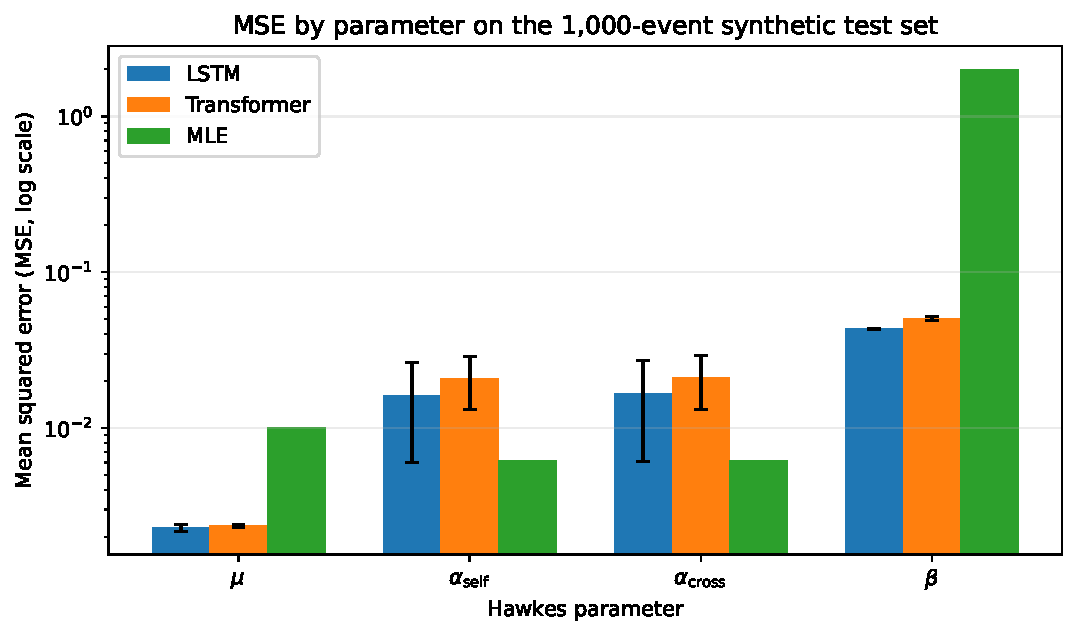
\includegraphics[width=\linewidth]{parameter_mse_en.pdf}
    \end{column}
  \end{columns}
\end{frame}

\begin{frame}{Backup: Lee's fixed point (mean / SD over 2,000 paths)}
  \scriptsize
  \begin{tabular}{lrrrrrrrr}
    \toprule
     & \multicolumn{2}{c}{\(\mu=0.3\)} & \multicolumn{2}{c}{\(\aself=0.4\)}
     & \multicolumn{2}{c}{\(\across=0.7\)} & \multicolumn{2}{c}{\(\beta=1.5\)}\\
    Estimator & Mean & SD & Mean & SD & Mean & SD & Mean & SD\\
    \midrule
    LSTM (ensemble) & 0.304 & 0.037 & 0.495 & 0.054 & 0.625 & 0.061 & 1.532 & 0.144\\
    Transformer (ensemble) & 0.296 & 0.039 & 0.528 & 0.056 & 0.606 & 0.062 & 1.531 & 0.154\\
    MLE (heuristic = oracle) & 0.307 & 0.037 & 0.396 & 0.073 & 0.708 & 0.086 & 1.516 & 0.164\\
    Lee (2023) network & 0.315 & 0.036 & 0.443 & 0.066 & 0.573 & 0.070 & 1.574 & 0.136\\
    Lee (2023) MLE & 0.304 & 0.031 & 0.399 & 0.050 & 0.702 & 0.061 & 1.508 & 0.115\\
    \bottomrule
  \end{tabular}
  \par\medskip
  \small Lee: 100,000 paths of 2,000 steps; here 2,000 paths of 1,000 events.
\end{frame}

\begin{frame}{Backup: October 2023 by volatility tercile}
  \small
  \begin{tabular}{lrrrr}
    \toprule
    Variant & All & Low vol. & Medium vol. & High vol.\\
    \midrule
    Training-label mean & 0.629 & 0.500 & 0.333 & 1.055\\
    LSTM, from scratch & 0.409 & 0.405 & 0.329 & 0.492\\
    Transformer, from scratch & 0.333 & 0.449 & 0.312 & 0.238\\
    LSTM, fine-tuned (selected) & 0.121 & 0.108 & 0.071 & 0.185\\
    Transformer, fine-tuned & 0.083 & 0.034 & 0.039 & 0.176\\
    \bottomrule
  \end{tabular}
  \par\medskip
  1,281 windows, MLE converged in all; weights stored before the test was opened.
\end{frame}

\begin{frame}{Backup: Hawkes volatility signature (test block)}
  \centering
  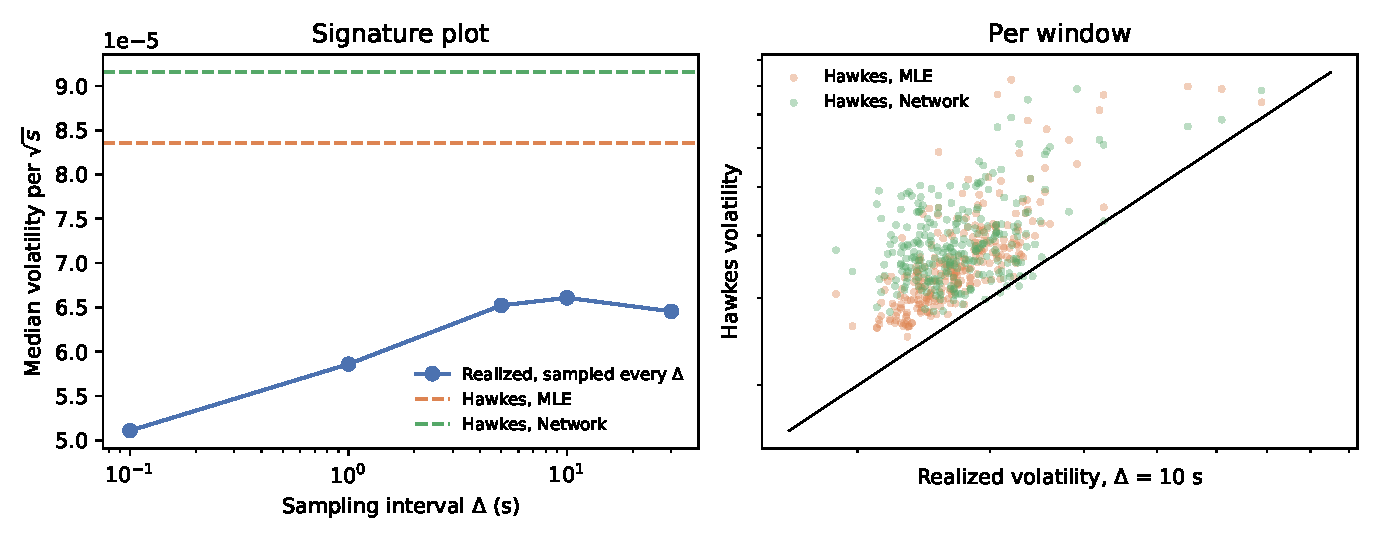
\includegraphics[width=0.8\linewidth]{hawkes_volatility_test.pdf}
\end{frame}

\end{document}
